\documentclass[tikz]{standalone}
\usetikzlibrary{calc}

\begin{document}

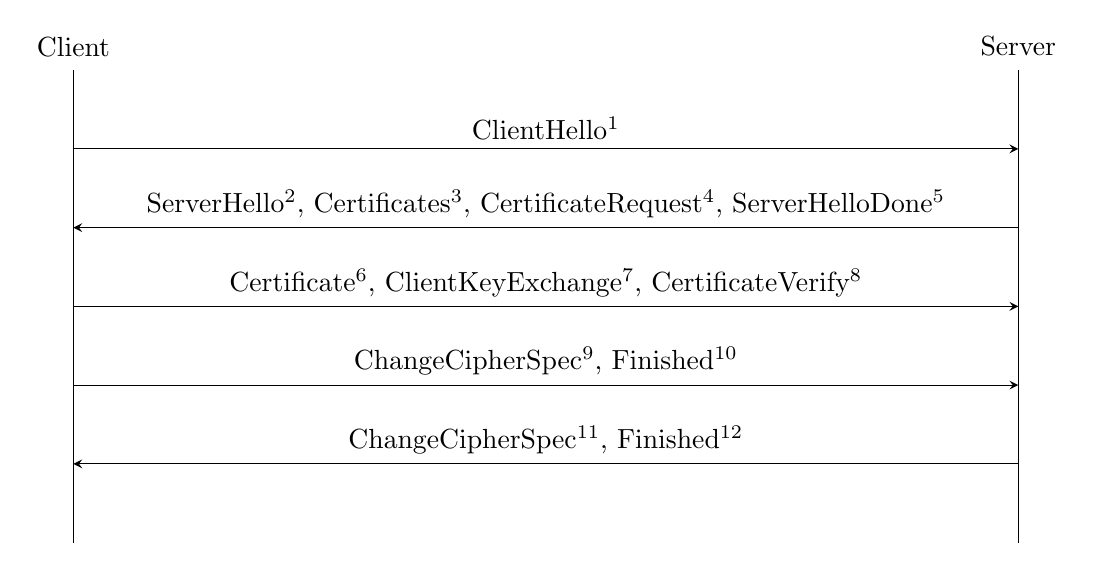
\begin{tikzpicture}
	\draw (-6,0) -- (-6,-6) (6,0) -- (6,-6);
	\node at (-6,.3) {Client};
	\node at (6,.3) {Server};

	\draw[-stealth] (-6,-1) -- node[midway,above] {ClientHello\footnote{1}} (6,-1);
	\draw[stealth-] (-6,-2) -- node[midway,above] {ServerHello\footnote{2}, Certificates\footnote{3}, CertificateRequest\footnote{4}, ServerHelloDone\footnote{5}} (6,-2);
	\draw[-stealth] (-6,-3) -- node[midway,above] {Certificate\footnote{6}, ClientKeyExchange\footnote{7}, CertificateVerify\footnote{8}} (6,-3);
	\draw[-stealth] (-6,-4) -- node[midway,above] {ChangeCipherSpec\footnote{9}, Finished\footnote{10}} (6,-4);
	\draw[stealth-] (-6,-5) -- node[midway,above] {ChangeCipherSpec\footnote{11}, Finished\footnote{12}} (6,-5);
\end{tikzpicture}

\end{document}

% \begin{tikzpicture}
% 	\draw (-3,0) -- (-3,-10) (3,0) -- (3,-10);
% 	\node at (-3,.3) {Client};
% 	\node at (3,.3) {Server};
% 
% 	\draw[-stealth] (-3,-1) -- node[midway,above] {ClientHello} (3,-1);
% 	\draw[stealth-] (-3,-2) -- node[midway,above] {ServerHello} (3,-2);
% 	\draw[stealth-] (-3,-3) -- node[midway,above] {Certificates} (3,-3);
% 	\draw[stealth-] (-3,-4) -- node[midway,above] {CertificateRequest} (3,-4);
% 	\draw[stealth-] (-3,-5) -- node[midway,above] {ServerHelloDone} (3,-5);
% 	\draw[-stealth] (-3,-6) -- node[midway,above] {Certificates} (3,-6);
% 	\draw[-stealth] (-3,-7) -- node[midway,above] {ClientKeyExchange} (3,-7);
% 	\draw[-stealth] (-3,-8) -- node[midway,above] {CertificateVerify} (3,-8);
% \end{tikzpicture}
